% Options for packages loaded elsewhere
% Options for packages loaded elsewhere
\PassOptionsToPackage{unicode}{hyperref}
\PassOptionsToPackage{hyphens}{url}
%
\documentclass[
  ignorenonframetext,
  aspectratio=169,
  russian,
]{beamer}
\newif\ifbibliography
\usepackage{pgfpages}
\setbeamertemplate{caption}[numbered]
\setbeamertemplate{caption label separator}{: }
\setbeamercolor{caption name}{fg=normal text.fg}
\beamertemplatenavigationsymbolshorizontal
% Prevent slide breaks in the middle of a paragraph
\widowpenalties 1 10000
\raggedbottom
\AtBeginPart{
  \frame{\partpage}
}
\AtBeginSection{
  \ifbibliography
  \else
    \frame{\sectionpage}
  \fi
}
\AtBeginSubsection{
  \frame{\subsectionpage}
}
\usepackage{iftex}
\ifPDFTeX
  \usepackage[T1]{fontenc}
  \usepackage[utf8]{inputenc}
  \usepackage{textcomp} % provide euro and other symbols
\else % if luatex or xetex
  \usepackage{unicode-math} % this also loads fontspec
  \defaultfontfeatures{Scale=MatchLowercase}
  \defaultfontfeatures[\rmfamily]{Ligatures=TeX,Scale=1}
\fi
\usepackage{lmodern}

\ifPDFTeX\else
  % xetex/luatex font selection
\fi
% Use upquote if available, for straight quotes in verbatim environments
\IfFileExists{upquote.sty}{\usepackage{upquote}}{}
\IfFileExists{microtype.sty}{% use microtype if available
  \usepackage[]{microtype}
  \UseMicrotypeSet[protrusion]{basicmath} % disable protrusion for tt fonts
}{}


\usepackage{longtable,booktabs,array}
\usepackage{calc} % for calculating minipage widths
\usepackage{caption}
% Make caption package work with longtable
\makeatletter
\def\fnum@table{\tablename~\thetable}
\makeatother
\usepackage{graphicx}
\makeatletter
\newsavebox\pandoc@box
\newcommand*\pandocbounded[1]{% scales image to fit in text height/width
  \sbox\pandoc@box{#1}%
  \Gscale@div\@tempa{\textheight}{\dimexpr\ht\pandoc@box+\dp\pandoc@box\relax}%
  \Gscale@div\@tempb{\linewidth}{\wd\pandoc@box}%
  \ifdim\@tempb\p@<\@tempa\p@\let\@tempa\@tempb\fi% select the smaller of both
  \ifdim\@tempa\p@<\p@\scalebox{\@tempa}{\usebox\pandoc@box}%
  \else\usebox{\pandoc@box}%
  \fi%
}
% Set default figure placement to htbp
\def\fps@figure{htbp}
\makeatother



\ifLuaTeX
\usepackage[bidi=basic,provide=*]{babel}
\else
\usepackage[bidi=default,provide=*]{babel}
\fi
% get rid of language-specific shorthands (see #6817):
\let\LanguageShortHands\languageshorthands
\def\languageshorthands#1{}


\setlength{\emergencystretch}{3em} % prevent overfull lines

\providecommand{\tightlist}{%
  \setlength{\itemsep}{0pt}\setlength{\parskip}{0pt}}



 

\usepackage[]{csquotes}

\IfFileExists{plex-otf.sty}{
  %% Full TeXlive
  % \usepackage[%
  %   % math,
  %   RM={Scale=0.94},SS={Scale=0.94},SScon={Scale=0.94},TT={Scale=MatchLowercase,FakeStretch=0.9},DefaultFeatures={Ligatures=Common}
  % ]{plex-otf}
}{
  %% TinyTeX
  \usepackage{libertine}
  \usepackage{juliamono}
}

%%% Load theme
% https://deic.uab.cat/~iblanes/beamer_gallery/
\IfFileExists{beamerthemegotham.sty}{
  %% Full TeXlive
  \usetheme{gotham}
  \gothamset{
    numbering=totalpagenumber,
    parttocframe default=off,
    sectiontocframe default=off,
    subsectiontocframe default=off,
  }
}{
  %% TinyTeX
  \usetheme{Madrid}
}
\makeatletter
\@ifpackageloaded{caption}{}{\usepackage{caption}}
\AtBeginDocument{%
\ifdefined\contentsname
  \renewcommand*\contentsname{Содержание}
\else
  \newcommand\contentsname{Содержание}
\fi
\ifdefined\listfigurename
  \renewcommand*\listfigurename{Список иллюстраций}
\else
  \newcommand\listfigurename{Список иллюстраций}
\fi
\ifdefined\listtablename
  \renewcommand*\listtablename{Список таблиц}
\else
  \newcommand\listtablename{Список таблиц}
\fi
\ifdefined\figurename
  \renewcommand*\figurename{Рисунок}
\else
  \newcommand\figurename{Рисунок}
\fi
\ifdefined\tablename
  \renewcommand*\tablename{Таблица}
\else
  \newcommand\tablename{Таблица}
\fi
}
\@ifpackageloaded{float}{}{\usepackage{float}}
\floatstyle{ruled}
\@ifundefined{c@chapter}{\newfloat{codelisting}{h}{lop}}{\newfloat{codelisting}{h}{lop}[chapter]}
\floatname{codelisting}{Список}
\newcommand*\listoflistings{\listof{codelisting}{Листинги}}
\makeatother
\makeatletter
\makeatother
\makeatletter
\@ifpackageloaded{caption}{}{\usepackage{caption}}
\@ifpackageloaded{subcaption}{}{\usepackage{subcaption}}
\makeatother

\usepackage{bookmark}
\IfFileExists{xurl.sty}{\usepackage{xurl}}{} % add URL line breaks if available
\urlstyle{same}
\hypersetup{
  pdftitle={Проектная работа. Образование планетной системы},
  pdfauthor={Арбатова Варвара Петровна; Карпова Есения Алексеевна; Дагделен Зейнап Реджеповна; Бюгданюк Анна Васильевна; Люпп Софья Романовна},
  pdflang={ru-RU},
  hidelinks,
  pdfcreator={LaTeX via pandoc}}


\title{Проектная работа. Образование планетной системы}
\subtitle{Второй этап}
\author{Арбатова Варвара Петровна \and Карпова Есения
Алексеевна \and Дагделен Зейнап Реджеповна \and Бюгданюк Анна
Васильевна \and Люпп Софья Романовна}
\date{2026-04-10}

\begin{document}
\frame{\titlepage}

\renewcommand*\contentsname{Содержание}
\begin{frame}[allowframebreaks]
  \frametitle{Содержание}
  \setcounter{tocdepth}{2}
  \tableofcontents
\end{frame}
\setcounter{tocdepth}{2}
\tableofcontents
}

\section{1. Цель
работы}\label{ux446ux435ux43bux44c-ux440ux430ux431ux43eux442ux44b}

\begin{frame}{1. Цель работы}
Целью данного этапа работы является разработка алгоритмов численного
моделирования образования планетной системы из газопылевого облака,
включая алгоритмы вычисления гравитационных сил, сил отталкивания и
трения, интегрирования уравнений движения, обновления угловых скоростей
и слипания частиц, на основе которых будет реализована программа
моделирования.
\end{frame}

\section{2. Структуры
данных}\label{ux441ux442ux440ux443ux43aux442ux443ux440ux44b-ux434ux430ux43dux43dux44bux445}

\begin{frame}{2. Структуры данных}
Каждая частица описывается набором параметров: масса \(m_i\), радиус
\(R_i\), координаты \(\mathbf{r}_i\), скорость \(\mathbf{v}_i\), угловая
скорость \(\omega_i\) и флаг активности (нужен для обработки слипания).
Все частицы хранятся в массиве фиксированной длины \(N\).

\begin{figure}

\centering{


\includegraphics[width=0.7\linewidth,height=\textheight,keepaspectratio]{image/1.png}

}

\caption{\label{fig-001}}

\end{figure}%
\end{frame}

\section{3. Инициализация}\label{ux438ux43dux438ux446ux438ux430ux43bux438ux437ux430ux446ux438ux44f}

\begin{frame}{3. Инициализация}
\[
r = r_0\sqrt{\xi_1}, \quad \alpha = 2\pi\,\xi_2
\]

\[
v_x = -y\,\omega_0\left(\frac{r_0}{r}\right)^{3/2}, \quad v_y = x\,\omega_0\left(\frac{r_0}{r}\right)^{3/2}, \quad v_z = 0
\]

\[
\mathbf{v}_i \leftarrow \mathbf{v}_i - \frac{\sum_j m_j \mathbf{v}_j}{\sum_j m_j}
\]
\end{frame}

\section{4. Главный
цикл}\label{ux433ux43bux430ux432ux43dux44bux439-ux446ux438ux43aux43b}

\begin{frame}{4.1 Шаг 1. Вычисление сил}
\phantomsection\label{ux448ux430ux433-1.-ux432ux44bux447ux438ux441ux43bux435ux43dux438ux435-ux441ux438ux43b}
\begin{figure}

\centering{


\includegraphics[width=0.5\linewidth,height=\textheight,keepaspectratio]{image/2.png}

}

\caption{\label{fig-001}}

\end{figure}%

\[
\mathbf{F}^g_{ij} = -\frac{\gamma m_i m_j}{b^3}\,\mathbf{b}_{ij}
\]

\[
\mathbf{F}^r_{ij} = k\left(\left(\frac{R_i+R_j}{b}\right)^8 - 1\right)\frac{\mathbf{b}_{ij}}{b}
\]

\[
W_\perp = (\mathbf{W} \cdot \mathbf{n}_{ij}) - \omega_i R_i - \omega_j R_j
\]

\[
\mathbf{F}^f_{ij} = \beta\,W_\perp\,F^r(b)\,\mathbf{n}_{ij}
\]
\end{frame}

\begin{frame}{4.2 Шаг 2. Интегрирование уравнений движения}
\phantomsection\label{ux448ux430ux433-2.-ux438ux43dux442ux435ux433ux440ux438ux440ux43eux432ux430ux43dux438ux435-ux443ux440ux430ux432ux43dux435ux43dux438ux439-ux434ux432ux438ux436ux435ux43dux438ux44f}

\includegraphics[width=0.5\linewidth,height=\textheight,keepaspectratio]{image/3.png}
\[
\mathbf{r}_i \leftarrow \mathbf{r}_i + \mathbf{v}_i\,\Delta t + \frac{\mathbf{F}_i}{2m_i}\,\Delta t^2
\]

\[
\mathbf{v}_i \leftarrow \mathbf{v}_i + \frac{\mathbf{F}_i^{\,\text{old}} + \mathbf{F}_i^{\,\text{new}}}{2m_i}\,\Delta t
\]
\end{frame}

\begin{frame}{4.3 Шаг 3. Обновление угловых скоростей}
\phantomsection\label{ux448ux430ux433-3.-ux43eux431ux43dux43eux432ux43bux435ux43dux438ux435-ux443ux433ux43bux43eux432ux44bux445-ux441ux43aux43eux440ux43eux441ux442ux435ux439}
\begin{figure}

\centering{


\includegraphics[width=0.5\linewidth,height=\textheight,keepaspectratio]{image/4.jpg}

}

\caption{\label{fig-001}}

\end{figure}%

\[
\varepsilon_i = \frac{1}{I_i}\sum_{j} \frac{b_{ij}}{R_i + R_j} F^f_{ij}, \quad I_i = \frac{2}{5}m_i R_i^2
\]

\[
\omega_i \leftarrow \omega_i + \varepsilon_i\,\Delta t
\]
\end{frame}

\begin{frame}{4.4 Шаг 4. Проверка условия слипания}
\phantomsection\label{ux448ux430ux433-4.-ux43fux440ux43eux432ux435ux440ux43aux430-ux443ux441ux43bux43eux432ux438ux44f-ux441ux43bux438ux43fux430ux43dux438ux44f}
Перебираются все активные пары \((i, j)\). Если \(b_{ij} < \delta\)
(пороговое расстояние), частицы объединяются: вычисляются параметры
новой частицы с сохранением массы и импульса:

\[
m \leftarrow m_i + m_j, \quad R \leftarrow \sqrt[3]{R_i^3 + R_j^3}
\]

\[
\mathbf{r} \leftarrow \frac{m_i\mathbf{r}_i + m_j\mathbf{r}_j}{m}, \quad \mathbf{v} \leftarrow \frac{m_i\mathbf{v}_i + m_j\mathbf{v}_j}{m}
\]

Результат записывается на место частицы \(i\), частица \(j\) помечается
как неактивная. Общее число активных частиц уменьшается на единицу.
\end{frame}

\begin{frame}{4.5 Шаг 5. Вычисление и запись энергий}
\phantomsection\label{ux448ux430ux433-5.-ux432ux44bux447ux438ux441ux43bux435ux43dux438ux435-ux438-ux437ux430ux43fux438ux441ux44c-ux44dux43dux435ux440ux433ux438ux439}
\[
E_k = \sum_i \frac{m_i v_i^2}{2} + \sum_i \frac{I_i \omega_i^2}{2}, \quad U = -\frac{1}{2}\sum_{i \neq j} \frac{\gamma m_i m_j}{b_{ij}}
\]

\[
E = E_k + U, \quad Q(t) = E(0) - E(t)
\]
\end{frame}

\section{5. Блок-схемы}\label{ux431ux43bux43eux43a-ux441ux445ux435ux43cux44b}

\begin{frame}{5. Блок-схемы}
\begin{figure}

\centering{

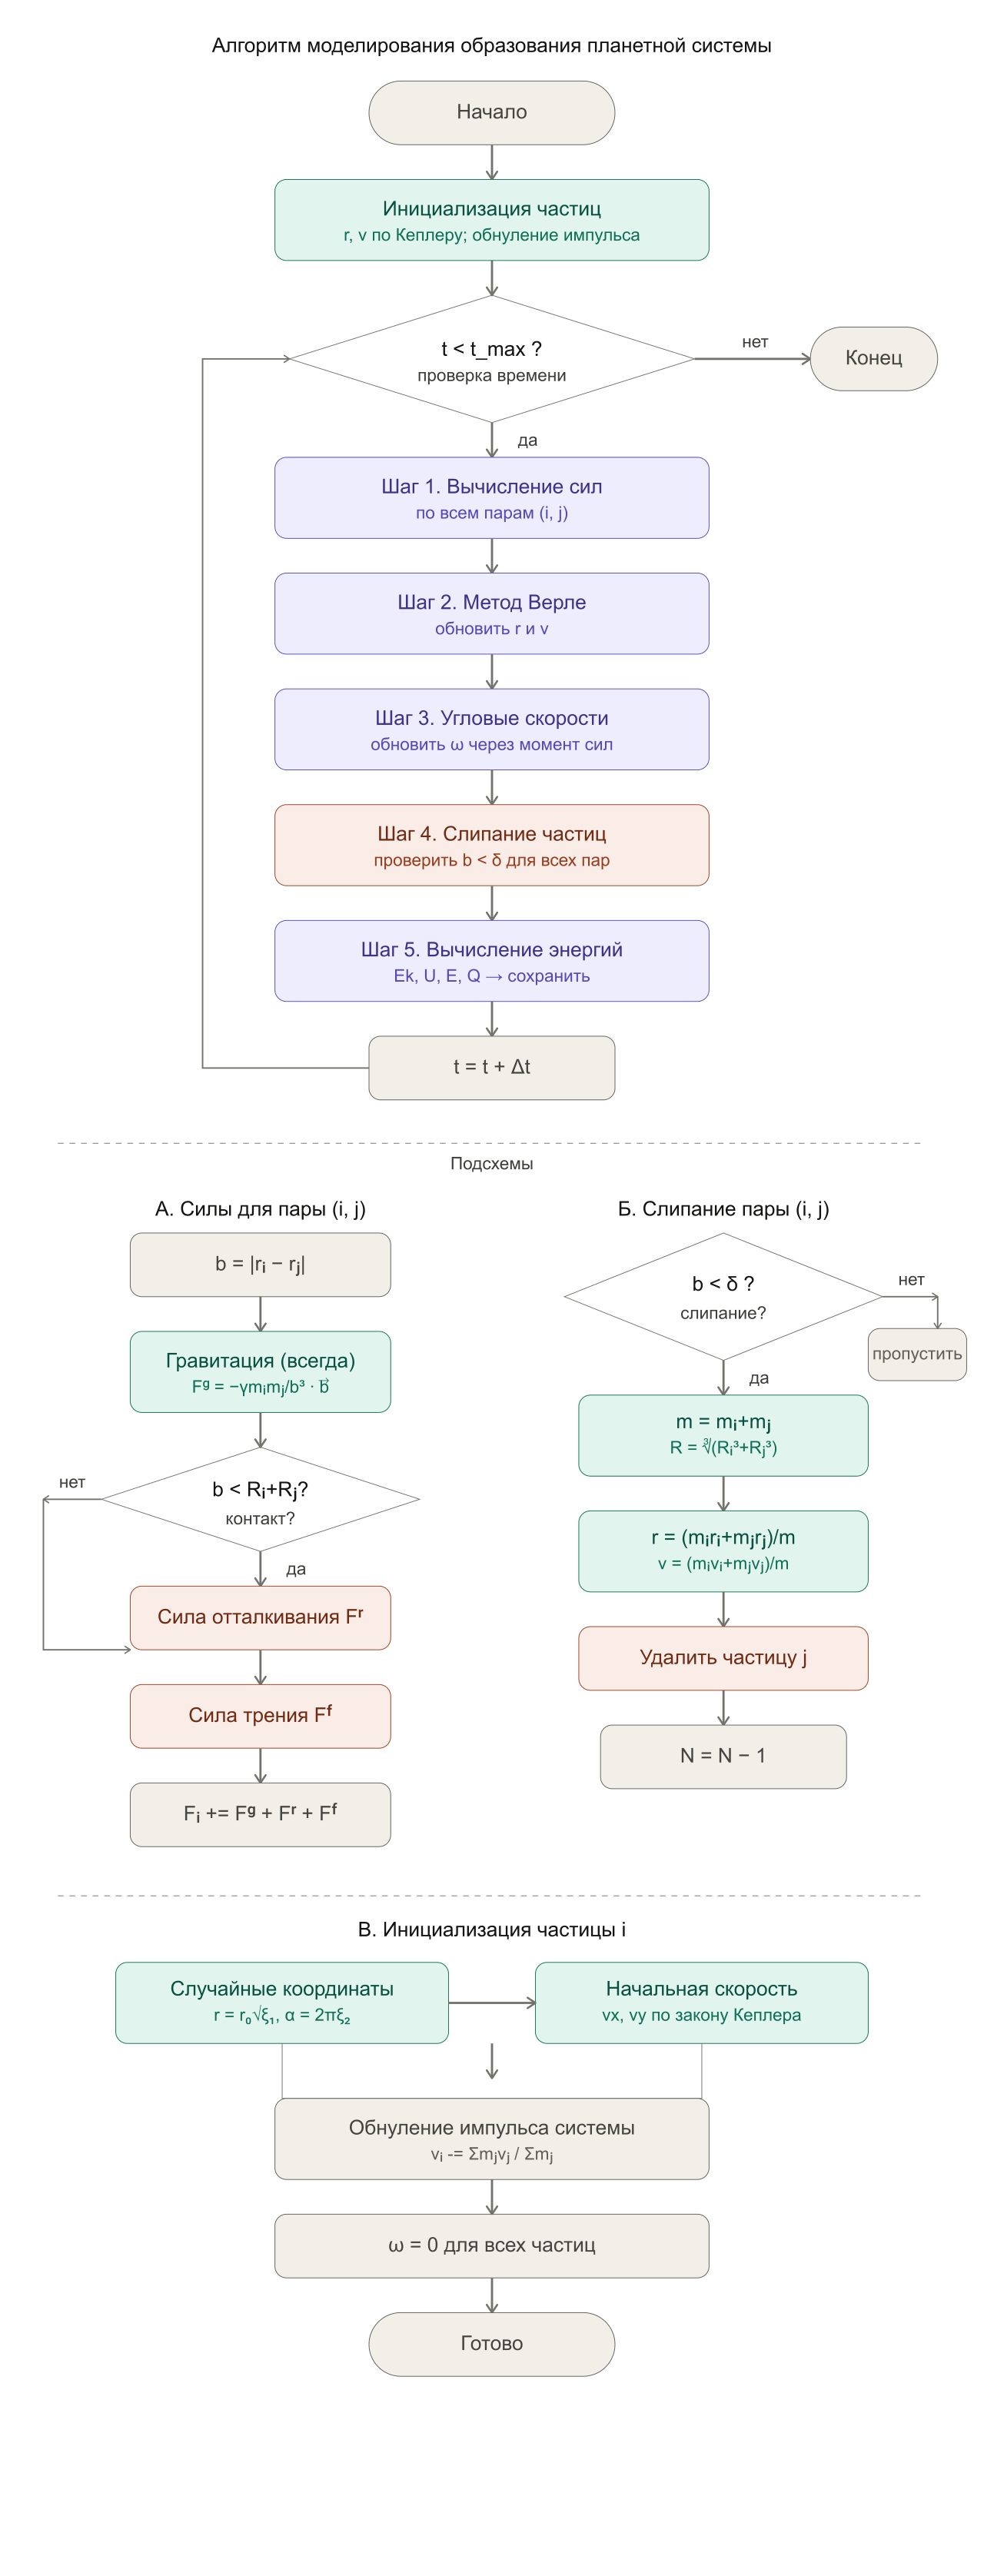
\includegraphics[width=0.7\linewidth,height=\textheight,keepaspectratio]{image/planetary_system_algorithm_flowchart.png}

}

\caption{\label{fig-001}Схема}

\end{figure}%
\end{frame}

\section{6. Вывод}\label{ux432ux44bux432ux43eux434}

\begin{frame}{6. Вывод}
На данном этапе были разработаны алгоритмы численного моделирования:
инициализация системы частиц, вычисление гравитационных сил, сил
отталкивания и трения, интегрирование уравнений движения методом Верле,
обновление угловых скоростей, слипание частиц с сохранением массы и
импульса, а также вычисление энергий системы. Полученные алгоритмы
служат основой для программной реализации на следующем этапе.

\phantomsection\label{refs}
\end{frame}




\end{document}
